% ===============================
%          Chapter 1.3
%          Factorising
%     Created by Michael Tang
%           2025.02.23
% ===============================

\subsection{Factorising}
Factorising involves writing an expression as a product of its factors. The process is the reverse expanding brackets.
\begin{figure}[H]
    \centering
    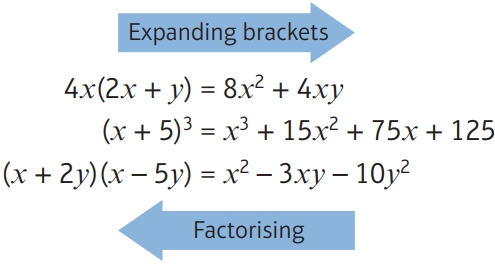
\includegraphics[scale=0.3]{Mathematics/Pure Mathematics/Ch1/Images/Ch1-3-1.png}
\end{figure}
\begin{itemize}
    \item Steps to Factorise:
    \begin{itemize}
        \item[1.] Identify the common factor in all terms of the expression and factor it out.
        \item[2.] For \underline{quadratic expressions} (二次表达式) like $ax^2 + bx + c$, find two numbers that multiply to give
        $ac$ and add to give $b$.
        \item[3.] Factorise the quadratic expression by breaking it into two \underline{binomials} (二项式).
    \end{itemize}
    \item Factorising Formulae
    \begin{itemize}
        \item \textbf{Common Factor}: To factor an expression by taking out the common factor:
        \begin{equation}
            ax + ay = a\left(x + y\right)
        \end{equation}
        \item \textbf{Quadratic Factorisation:} For a quadratic expression $ax^2 + bx + c$, find two numbers that:
        \begin{itemize}
            \item Multiply to $ac$ (the product of $a$ and $c$).
            \item Add up to $b$ (the coefficient of the middle term).
        \end{itemize}
        The rewrite the middle term using these two numbers and factor by grouping. Formula:
        \begin{equation}
            ax^2 + bx + c = a\left(x + p\right)\left(x + q\right)
        \end{equation}
        where $p$ and $q$ are the factors of $ac$ that add up to $b$.
        \item \textbf{Difference of Squares:} The difference of squares formula is used when you have an expression like
        $a^2 - b^2$. It can be factored as:
        \begin{equation}
            a^2 - b^2 = \left(a + b\right)\left(a - b\right)
        \end{equation}
        \item \textbf{Perfect Square Trinomial:} For expressions of the form $a^2 \pm 2ab + b^2$, it factors into a perfect
        square:
        \begin{equation}
            a^2 \pm 2ab + b^2 = \left(a \pm b\right)^2
        \end{equation}
        \item \textbf{Factorising by Grouping:} When you have four terms, factor by grouping:
        \begin{equation}
            ax + bx + ay + by = \left(a + b\right)\left(x + y\right)
        \end{equation}
        \item \textbf{Factorising Quadratics by Completing the Square (for advanced problems):} For a quadratic expression of the
        form $ax^2 + bx + c$, it can sometimes be completed into a perfect square for easy factorisation.
        \begin{equation}
            ax^2 + bx + c = a \left(x^2 + \frac{b}{a} x + \left(\frac{b}{2a}\right)^2\right) - a \left(\frac{b}{2a}\right)^2 + c
        \end{equation}
    \end{itemize}
\end{itemize}